%----------------------------------------------------------------------------------------
%	PACKAGES AND THEMES
%----------------------------------------------------------------------------------------
\documentclass[aspectratio=169,xcolor=dvipsnames]{beamer}
\usetheme{Simple}

\usepackage{hyperref}
\usepackage{graphicx} % Allows including images
\usepackage{booktabs} % Allows the use of \toprule, \midrule and \bottomrule in tables
\usepackage{graphicx}
\usepackage{amsmath}

\usepackage{mathtools}% superior to amsmath
\usepackage{tikz}
\usepackage{animate}

\makeatletter
\newcommand\mathcircled[1]{%
  \mathpalette\@mathcircled{#1}%
}
\newcommand\@mathcircled[2]{%
  \tikz[baseline=(math.base)] \node[draw,circle,inner sep=15pt] (math) {$\m@th#1#2$};%
}
\makeatother
%----------------------------------------------------------------------------------------
%	TITLE PAGE
%----------------------------------------------------------------------------------------

% The title
\title[short title]{Simple Beamer Theme}
\subtitle{Lecture 13}

\author[Narek Maloyan] {Narek Maloyan}
\institute[NTU] % Your institution may be shorthand to save space
{
    % Your institution for the title page
    Faculty of Computational Mathematics and Cybernetics \\
    Lomonosov Moscow State University
    \vskip 3pt
}
\date{\today} % Date, can be changed to a custom date


%----------------------------------------------------------------------------------------
%	PRESENTATION SLIDES
%----------------------------------------------------------------------------------------

\begin{document}

\begin{frame}
    % Print the title page as the first slide
    \titlepage
\end{frame}

\begin{frame}{Overview}
    % Throughout your presentation, if you choose to use \section{} and \subsection{} commands, these will automatically be printed on this slide as an overview of your presentation
    \tableofcontents
\end{frame}

%------------------------------------------------
\section{What is neuron?}
%------------------------------------------------

\begin{frame}{Neuron}
    $$\mathcircled{0.4}$$
    \begin{center}
        \textbf{Neuron} $\rightarrow$ Thing that holds a number       
    \end{center}
\end{frame}

\begin{frame}{Activation map}
    \begin{center}
        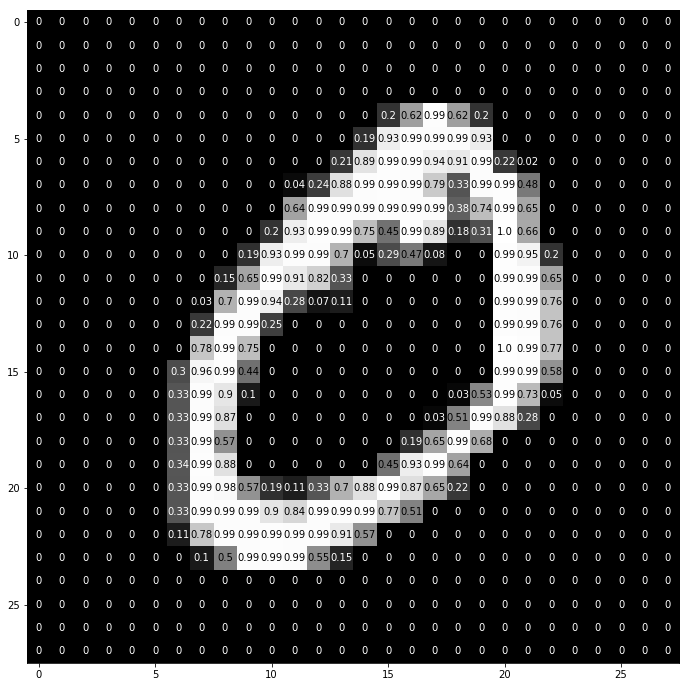
\includegraphics[width=0.8\textheight]{../images/mnist_cnn_keras_8_0.png}
    \end{center}
\end{frame}

\begin{frame}{Forward pass}
    \begin{center}
        \animategraphics[loop,controls,width=\textheight]{10}{../images/nn_animation-}{0}{107}
    \end{center}
\end{frame}

%------------------------------------------------
\section{What is intelligence?}
%------------------------------------------------
\begin{frame}{Patterns}
    \begin{center}
        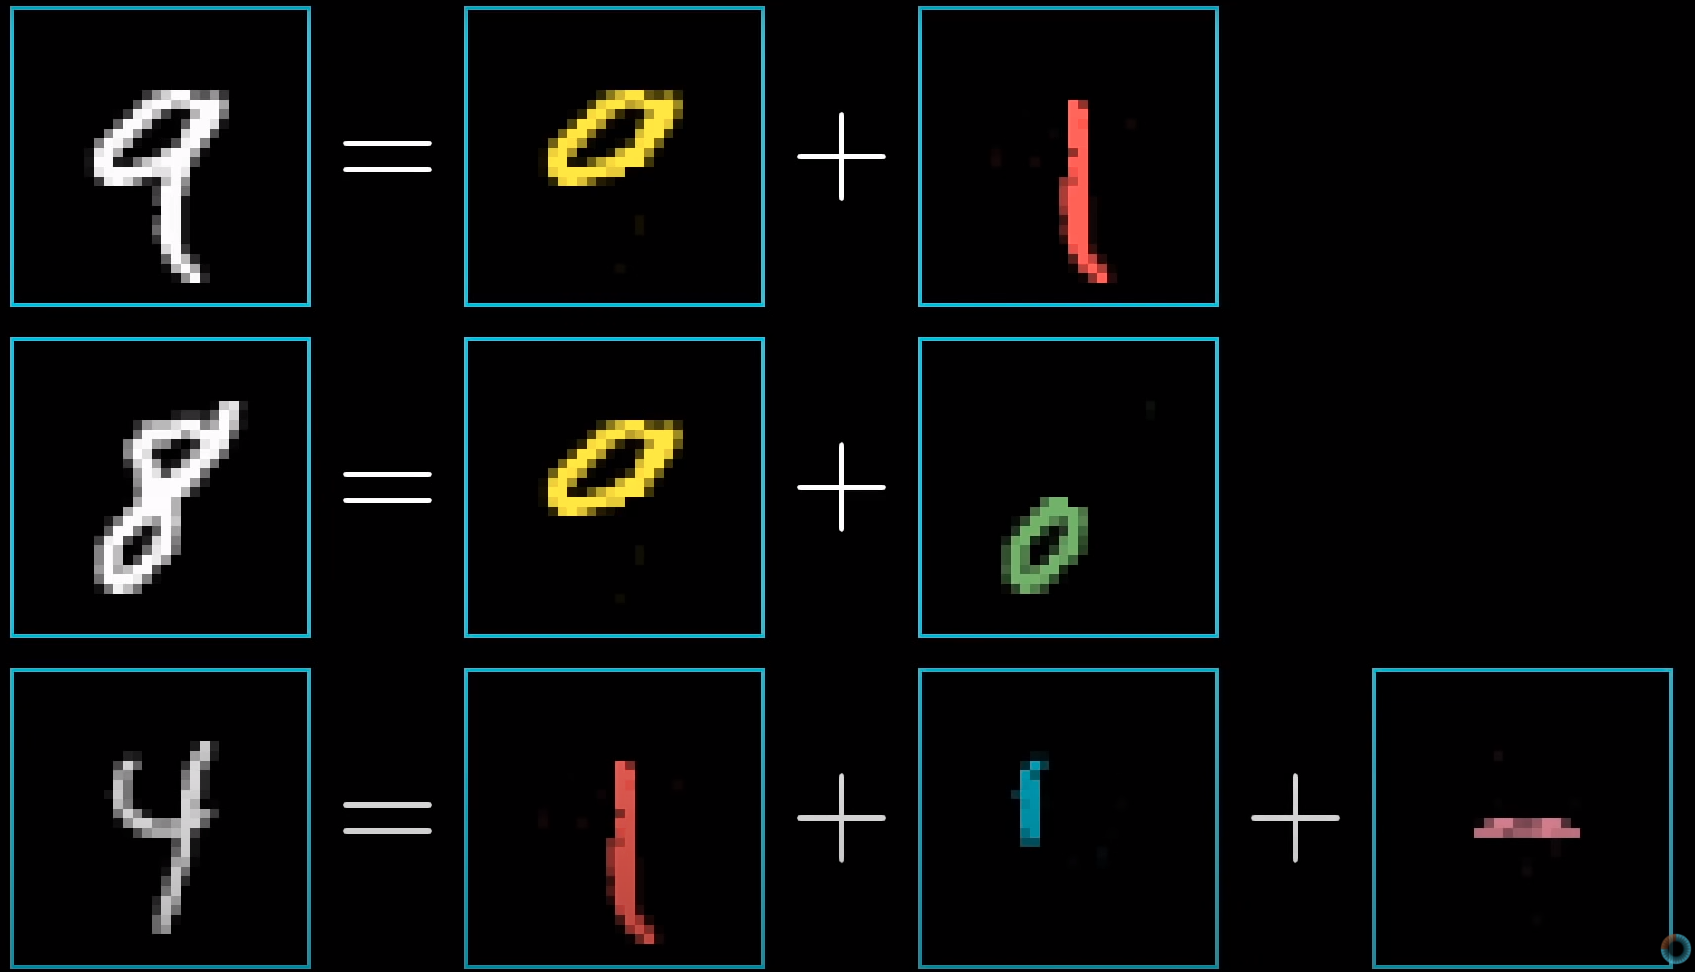
\includegraphics[width=\textheight]{../images/patterns.png}
    \end{center}
\end{frame}

%------------------------------------------------
\section{Neural network}
%------------------------------------------------
\begin{frame}{General formula}
    $$f = \sigma (Wx + b)$$
    \begin{center}
        $W$ - Weights \\
        $b$ - Biases  \\
        $x$ - Input \\
        $\sigma$ - Activation function            
    \end{center}
\end{frame}

\begin{frame}{Formula}
    \begin{center}
        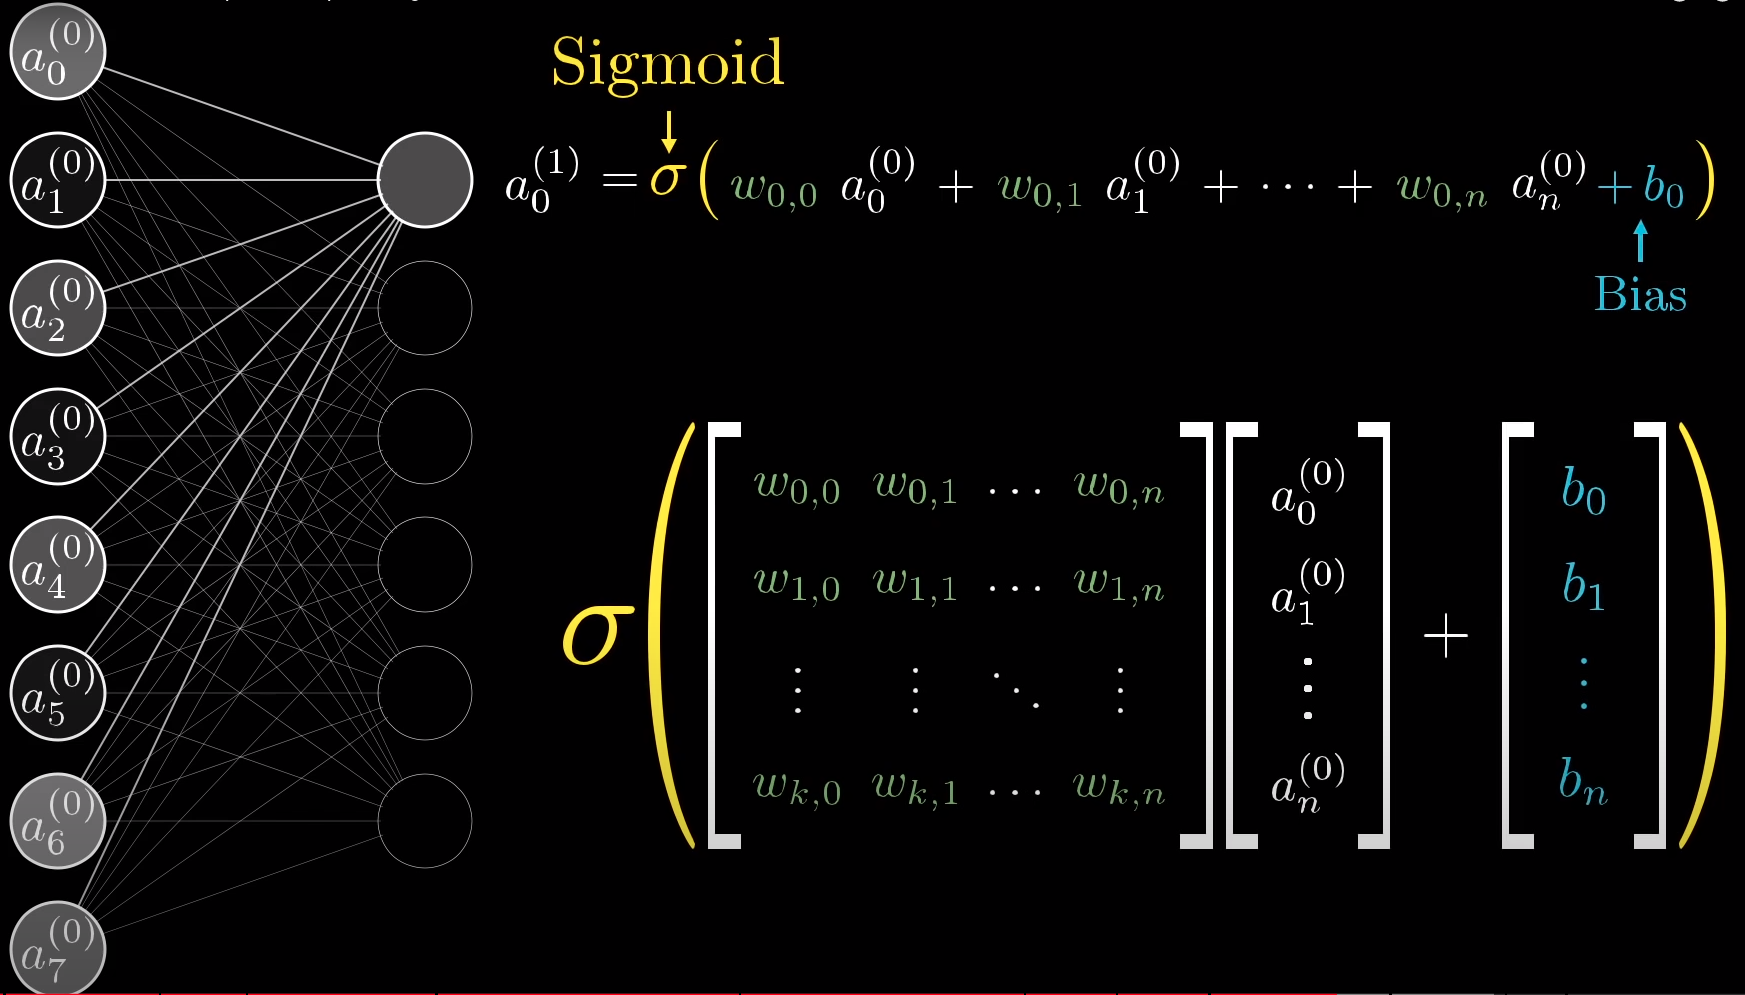
\includegraphics[width=1.5\textheight]{../images/formula.png}
    \end{center}
\end{frame}

%------------------------------------------------

%------------------------------------------------
\section{Universal approximation theorem}
%------------------------------------------------
\begin{frame}{Universal approximation theorem}
    \begin{theorem}[UAT interpretation for NN]
       2-layer NNs with sigmoid activation function can approximate any other function
    \end{theorem}
\end{frame}
%------------------------------------------------

\begin{frame}{Can we use just 1 layer?}
    \begin{center}
        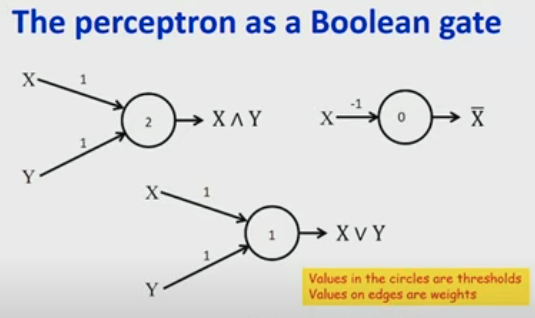
\includegraphics[width=1.3\textheight]{../images/perceptron_as_a_boolean_gate.png}
    \end{center}
\end{frame}

%------------------------------------------------
\section{Second Section}
%------------------------------------------------

\begin{frame}{Can we use just 1 layer?}
    No, we can't. For example, XOR
\end{frame}

%------------------------------------------------

\begin{frame}{Theorem}
    \begin{theorem}[Mass--energy equivalence]
        $E = mc^2$
    \end{theorem}
\end{frame}

%------------------------------------------------

\begin{frame}{Figure}
    Uncomment the code on this slide to include your own image from the same directory as the template .TeX file.
    %\begin{figure}
    %\includegraphics[width=0.8\linewidth]{test}
    %\end{figure}
\end{frame}

%------------------------------------------------

\begin{frame}[fragile] % Need to use the fragile option when verbatim is used in the slide
    \frametitle{Citation}
    An example of the \verb|\cite| command to cite within the presentation:\\~

    This statement requires citation \cite{p1}.
\end{frame}

%------------------------------------------------

\begin{frame}{References}
    % Beamer does not support BibTeX so references must be inserted manually as below
    \footnotesize{
        \begin{thebibliography}{99}
            \bibitem[Smith, 2012]{p1} John Smith (2012)
            \newblock Title of the publication
            \newblock \emph{Journal Name} 12(3), 45 -- 678.
        \end{thebibliography}
    }
\end{frame}

%------------------------------------------------

\begin{frame}
    \Huge{\centerline{The End}}
\end{frame}

%----------------------------------------------------------------------------------------

\end{document}